%% Creator: Inkscape inkscape 0.92.2, www.inkscape.org
%% PDF/EPS/PS + LaTeX output extension by Johan Engelen, 2010
%% Accompanies image file 'ykmae1.eps' (pdf, eps, ps)
%%
%% To include the image in your LaTeX document, write
%%   \input{<filename>.pdf_tex}
%%  instead of
%%   \includegraphics{<filename>.pdf}
%% To scale the image, write
%%   \def\svgwidth{<desired width>}
%%   \input{<filename>.pdf_tex}
%%  instead of
%%   \includegraphics[width=<desired width>]{<filename>.pdf}
%%
%% Images with a different path to the parent latex file can
%% be accessed with the `import' package (which may need to be
%% installed) using
%%   \usepackage{import}
%% in the preamble, and then including the image with
%%   \import{<path to file>}{<filename>.pdf_tex}
%% Alternatively, one can specify
%%   \graphicspath{{<path to file>/}}
%% 
%% For more information, please see info/svg-inkscape on CTAN:
%%   http://tug.ctan.org/tex-archive/info/svg-inkscape
%%
\begingroup%
  \makeatletter%
  \providecommand\color[2][]{%
    \errmessage{(Inkscape) Color is used for the text in Inkscape, but the package 'color.sty' is not loaded}%
    \renewcommand\color[2][]{}%
  }%
  \providecommand\transparent[1]{%
    \errmessage{(Inkscape) Transparency is used (non-zero) for the text in Inkscape, but the package 'transparent.sty' is not loaded}%
    \renewcommand\transparent[1]{}%
  }%
  \providecommand\rotatebox[2]{#2}%
  \ifx\svgwidth\undefined%
    \setlength{\unitlength}{395.9999901bp}%
    \ifx\svgscale\undefined%
      \relax%
    \else%
      \setlength{\unitlength}{\unitlength * \real{\svgscale}}%
    \fi%
  \else%
    \setlength{\unitlength}{\svgwidth}%
  \fi%
  \global\let\svgwidth\undefined%
  \global\let\svgscale\undefined%
  \makeatother%
  \begin{picture}(1,0.833939)%
    \put(0,0){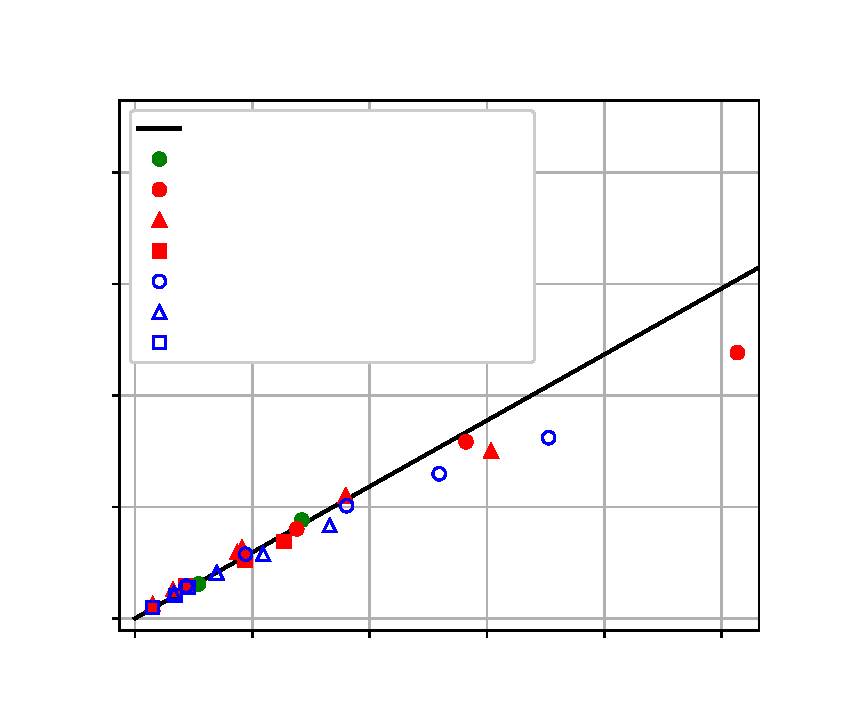
\includegraphics[width=\unitlength]{images_2ddl/ykmae1.eps}}%
    \put(0.14153535,0.05494683){\color[rgb]{0,0,0}\makebox(0,0)[lb]{\smash{0}}}%
    \put(0.26236869,0.05494683){\color[rgb]{0,0,0}\makebox(0,0)[lb]{\smash{500}}}%
    \put(0.39123232,0.05494683){\color[rgb]{0,0,0}\makebox(0,0)[lb]{\smash{1000}}}%
    \put(0.52812626,0.05494683){\color[rgb]{0,0,0}\makebox(0,0)[lb]{\smash{1500}}}%
    \put(0.6650202,0.05494683){\color[rgb]{0,0,0}\makebox(0,0)[lb]{\smash{2000}}}%
    \put(0.80191162,0.05494683){\color[rgb]{0,0,0}\makebox(0,0)[lb]{\smash{2500}}}%
    \put(0.06,0.09675819){\color[rgb]{0,0,0}\makebox(0,0)[lb]{\smash{0.0}}}%
    \put(0.06,0.23034304){\color[rgb]{0,0,0}\makebox(0,0)[lb]{\smash{5.0}}}%
    \put(0.045109697,0.365){\color[rgb]{0,0,0}\makebox(0,0)[lb]{\smash{10.0}}}%
    \put(0.045109697,0.505){\color[rgb]{0,0,0}\makebox(0,0)[lb]{\smash{15.0}}}%
    \put(0.045109697,0.645){\color[rgb]{0,0,0}\makebox(0,0)[lb]{\smash{20.0}}}%
    \put(0.025,0.33304759){\color[rgb]{0,0,0}\rotatebox{90}{\makebox(0,0)[lb]{\smash{$H_{max}/R$}}}}%
    \put(0.21843434,0.6914693){\color[rgb]{0,0,0}\makebox(0,0)[lb]{\smash{\small modèle théorique 2DDL}}}%
    \put(0.21843434,0.65442132){\color[rgb]{0,0,0}\makebox(0,0)[lb]{\smash{\small Y\&K acier (120,30)}}}%
    \put(0.21843434,0.61737082){\color[rgb]{0,0,0}\makebox(0,0)[lb]{\smash{\small Y\&K polyimide (125,10)}}}%
    \put(0.21843434,0.58032031){\color[rgb]{0,0,0}\makebox(0,0)[lb]{\smash{\small Y\&K polyimide (125,15)}}}%
    \put(0.21843434,0.54326981){\color[rgb]{0,0,0}\makebox(0,0)[lb]{\smash{\small Y\&K polyimide (125,20)}}}%
    \put(0.21843434,0.5062193){\color[rgb]{0,0,0}\makebox(0,0)[lb]{\smash{\small Y\&K polyimide (75,10)}}}%
    \put(0.21843434,0.4691688){\color[rgb]{0,0,0}\makebox(0,0)[lb]{\smash{\small Y\&K polyimide (75,15)}}}%
    \put(0.21843434,0.43211829){\color[rgb]{0,0,0}\makebox(0,0)[lb]{\smash{\small Y\&K polyimide (75,25)}}}%
    \put(0.4,0.01){\color[rgb]{0,0,0}\makebox(0,0)[lb]{\smash{ $F^2 R/(E \rho g I A)$}}}%
  \end{picture}%
\endgroup%
